\chapter{Mitosis and Meiosis}\label{mitosis-and-meiosis}

\href{https://en.wikipedia.org/wiki/Mitosis}{Mitosis} is the part of the
cell cycle when replicated chromosomes are separated into two new
nuclei. In general, mitosis (division of the nucleus) is preceded by the
S stage of interphase (during which the DNA is replicated) and is often
accompanied or followed by cytokinesis, which divides the cytoplasm,
organelles and cell membrane into two new cells containing roughly equal
shares of these cellular components. Mitosis and cytokinesis together
define the mitotic (M) phase of an animal cell cycle (the division of
the mother cell into two daughter cells geneically identical to each
other). The process of mitosis is divided into stages corresponding to
the completion of one set of activities and the start of the next. These
stages are prophase, pro-metaphase, metaphase, anaphase, and telophase.

\href{https://en.wikipedia.org/wiki/Meiosis}{Meiosis} is a specialized
type of cell division that reduces the chromosome number by half,
creating four haploid cells, each genetically distinct from the parent
cell that gave rise to them. This process occurs in all sexually
reproducing single-celled and multicellular eukaryotes, including
animals, plants, and fungi. Errors in meiosis resulting in aneuploidy
are the leading known cause of miscarriage and the most frequent genetic
cause of developmental disabilities. In meiosis, DNA replication is
followed by two rounds of cell division to produce four daughter cells,
each with half the number of chromosomes as the original parent cell.
The two meiotic divisions are known as Meiosis I and Meiosis II. Before
meiosis begins, during S phase of the cell cycle, the DNA of each
chromosome is replicated so that it consists of two identical sister
chromatids, which remain held together through sister chromatid
cohesion. This S-phase can be referred to as ``premeiotic S-phase'' or
``meiotic S-phase''. Immediately following DNA replication, meiotic
cells enter a prolonged G2-like stage known as meiotic prophase. During
this time, homologous chromosomes pair with each other and undergo
genetic recombination, a programmed process in which DNA is cut and then
repaired, which allows them to exchange some of their genetic
information. A subset of recombination events results in crossovers,
which create physical links known as chiasmata (singular: chiasma, for
the Greek letter Chi (X)) between the homologous chromosomes. In most
organisms, these links are essential to direct each pair of homologous
chromosomes to segregate away from each other during Meiosis I,
resulting in two haploid cells that have half the number of chromosomes
as the parent cell. During Meiosis II, the cohesion between sister
chromatids is released and they segregate from one another, as during
mitosis. In some cases, all four of the meiotic products form gametes
such as sperm, spores, or pollen. In female animals, three of the four
meiotic products are typically eliminated by extrusion into polar
bodies, and only one cell develops to produce an ovum. Because the
number of chromosomes is halved during meiosis, gametes can fuse
(i.e.~fertilization) to form a diploid zygote that contains two copies
of each chromosome, one from each parent. Thus, alternating cycles of
meiosis and fertilization enable sexual reproduction, with successive
generations maintaining the same number of chromosomes. For example,
diploid human cells contain 23 pairs of chromosomes including 1 pair of
sex chromosomes (46 total), half of maternal origin and half of paternal
origin. Meiosis produces haploid gametes (ova or sperm) that contain one
set of 23 chromosomes. When two gametes (an egg and a sperm) fuse, the
resulting zygote is once again diploid, with the mother and father each
contributing 23 chromosomes. This same pattern, but not the same number
of chromosomes, occurs in all organisms that utilize meiosis.

\section{View Prepared Slides}\label{view-prepared-slides-1}

\begin{enumerate}
\def\labelenumi{\arabic{enumi}.}
\tightlist
\item
  View the onion root tip and observe the different stages of mitosis
  (Figure \ref{fig:tip}).
\end{enumerate}

\begin{figure}

{\centering 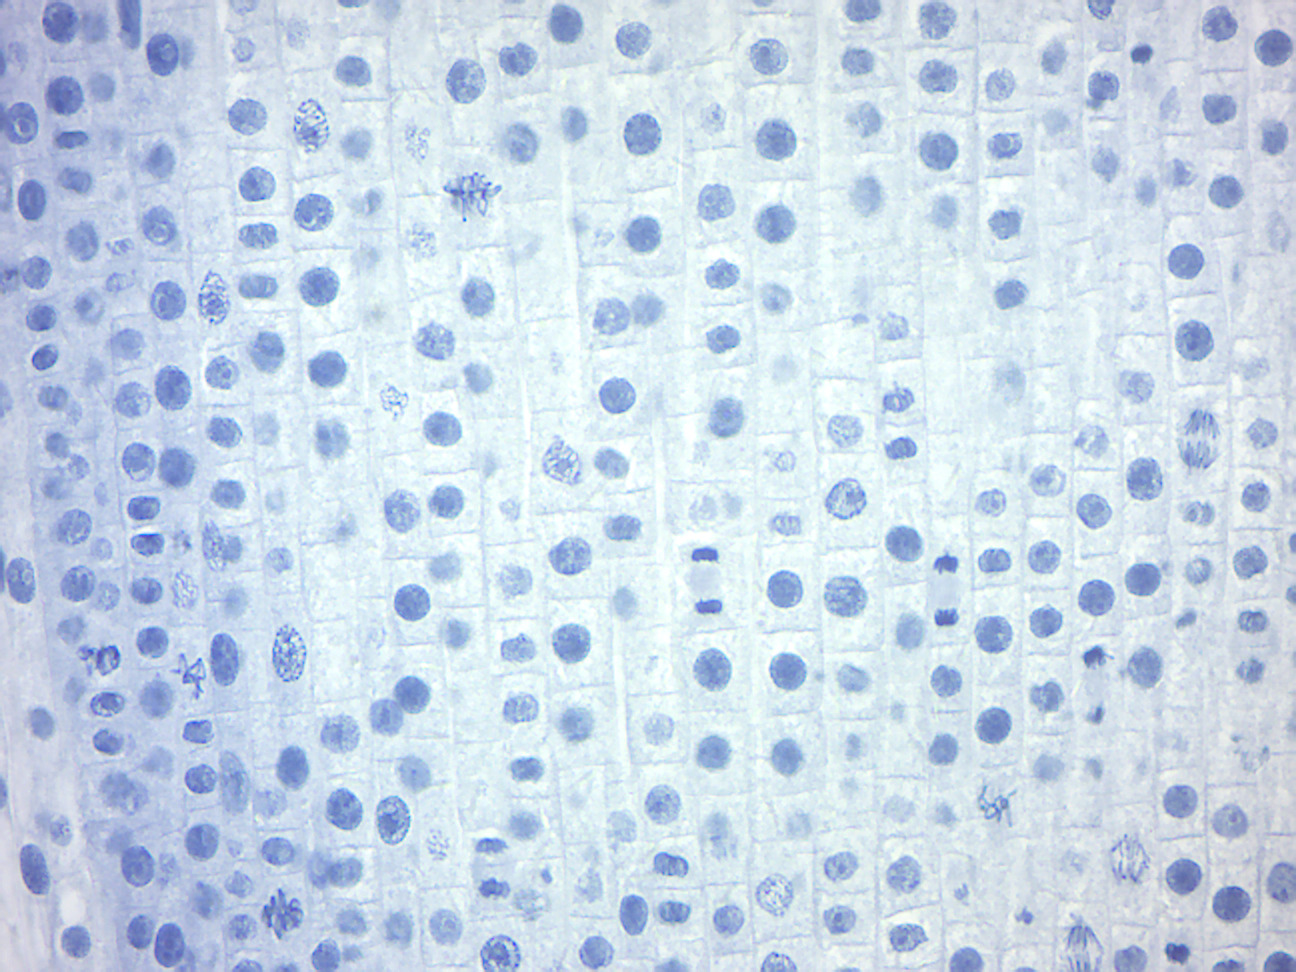
\includegraphics[width=0.7\linewidth]{./figures/mitosis/Onion_root_tip}

}

\caption{Onion root tip}\label{fig:tip}
\end{figure}

\begin{enumerate}
\def\labelenumi{\arabic{enumi}.}
\setcounter{enumi}{1}
\tightlist
\item
  View the fish blastodisc and observe the different stages of mitosis
  (Figure \ref{fig:blastodisc}).
\end{enumerate}

\begin{figure}

{\centering 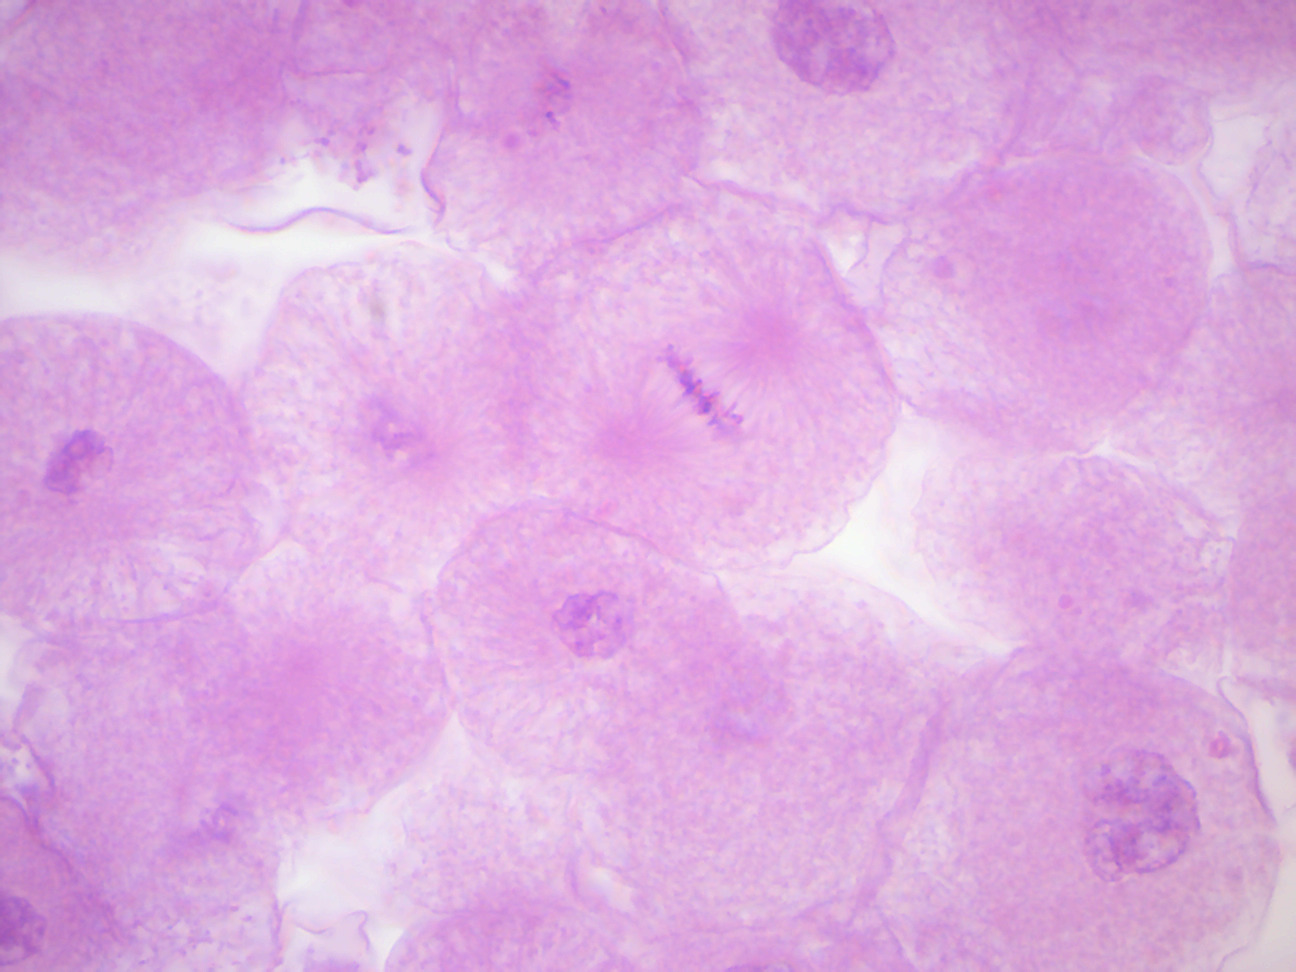
\includegraphics[width=0.7\linewidth]{./figures/mitosis/Fish_blastodisc}

}

\caption{Fish blastodisc}\label{fig:blastodisc}
\end{figure}

\section{Preparing an Onion root tip
squash}\label{preparing-an-onion-root-tip-squash}

\subsection{Experimental procedures}\label{experimental-procedures-25}

\begin{enumerate}
\def\labelenumi{\arabic{enumi}.}
\tightlist
\item
  Obtain an onion bulb that shows some roots.
\item
  Cut off a root tip and place it on a clean slide.
\item
  Cut off 1mm to 2mm of the root tip and throw away the upper portion of
  the root.
\item
  Cover the root tip with four drops of 1 N HCl and warm the slide over
  an alcohol burner flame for 1 minute. Do not boil.
\item
  Blot off the excess HCl and cover the root tip with 0.5\% aqueous
  toluidine blue.
\item
  Again, pass the slide through the alcohol burner flame for 1 minute
  without boiling.
\item
  Blot off the excess stain, add a drop of fresh stain, and apply a
  coverslip.
\item
  Cover the slide with a paper towel and carefully squash the coverslip
  firmly with your thumb.
\item
  Examine the slide for the stages of mitosis as well as interphase and
  cytokinesis.
\end{enumerate}

\begin{figure}

{\centering 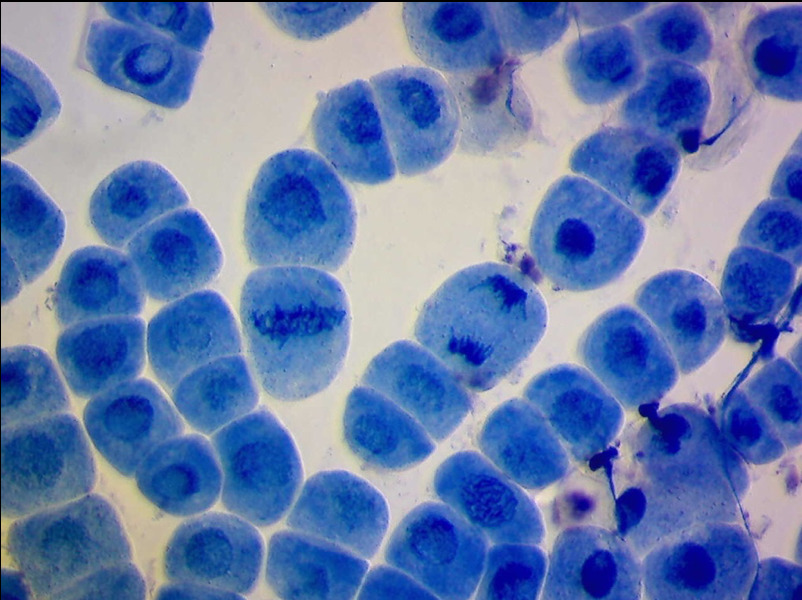
\includegraphics[width=0.7\linewidth]{./figures/mitosis/Onion_root_tip_spread}

}

\caption{Several different phases of mitosis are visible in this onion root tip spread.}\label{fig:spread}
\end{figure}

\section{Review Questions}\label{review-questions-6}

\begin{enumerate}
\def\labelenumi{\arabic{enumi}.}
\tightlist
\item
  What is mitosis and what is its outcome?
\item
  What is meiosis and what is its outrcome?
\item
  What is homologous recombination and what is its outcome?
\item
  What do the terms haploid and diploid mean?
\item
  Are you a haploid or a diploid organism?
\item
  What are gametes?
\item
  What is a zygote?
\end{enumerate}
